% \documentclass[UTF8,oneside]{ctexbook}
% \usepackage{pgfplots}
% \usepackage{caption}
% \begin{document}
% 这本书是关于软件设计的:如何将复杂的软件系统分解成模块(如类和方法),以便这些模块可以相对独立地实现。首先,这本书介绍了软件设计的基本问题,也就是对复杂性的管理。然后,它讨论了关于如何处理软件设计过程的一些哲学问题,并提出了一系列可以在软件设计过程中应用的设计原则。本书还介绍了一些可用来识别设计问题的危险信号。您可以通过应用本书中的想法来减少大型软件系统的复杂性,以便您可以更快和更低成本地编写软件。

\begin{figure}[!h]
% \centering

\makebox[\textwidth][c]{%
    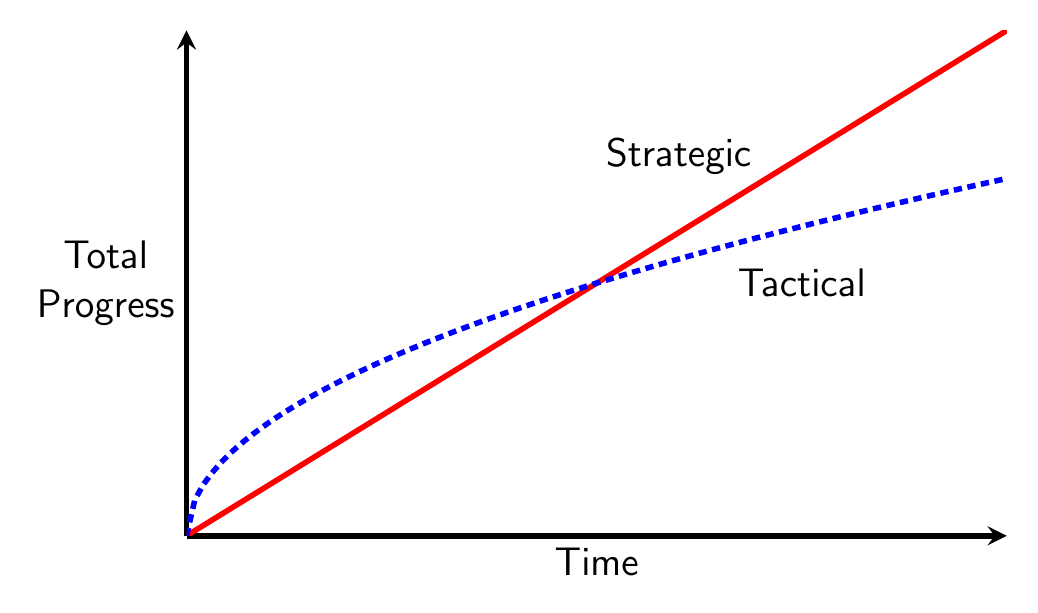
\begin{tikzpicture}[
        font = \sffamily\Large,
        every path/.append style ={line width = 2pt,},
    ]
    \begin{axis}[
        width = 12cm,
        height = 8cm,
        ticks = none,
        axis lines = left,
        xlabel = { Time } ,
        ylabel = { Total\\Progress },
        ylabel style = { rotate = -90, align  = center,},
    ]
    \addplot [domain=0:2,samples=100,color=red ] {x};
    \addplot [
        domain  = 0:2,
        samples = 100,
        color   = blue,
        densely dashed
    ] {x^0.5};
    \node[] at (axis cs: 1.2,1.5) { Strategic};
    \node[] at (axis cs: 1.5,1.0) { Tactical };
    \end{axis}
    \end{tikzpicture}
}%

\caption*{图 3.1}
\label{fig:3-1}
\end{figure}

% \end{document}